\section{Minkowski Functionals}
\label{sec:minkowski_functionals}
Minkowski functionals are powerful morphological descriptors derived from integral geometry, widely used to quantify the geometry and topology of spatial structures in cosmological datasets. 
Here, we will review \citet{2010PhRvD..81h3505M}, \citet{2012PhRvD..85j3513K} and \citet{2013PhRvD..88l3002P} for a comprehensive understanding of Minkowski functionals and their applications in cosmology.

\subsection{Definition}
Given a two-dimensional random field $\kappa(\hat{\mathbf{n}})$ (in our case, the convergence field) with zero mean and variance $\kappa^2 = \sigma_0^2$, we can consider its excursion sets $\Sigma(\nu) = \{ \kappa > \nu \sigma_0 \}$ which consist of all the points at which the field exceeds a particular threshold value $\nu \sigma_0$. 
Figure~\ref{fig:excursion_sets} depicts the excursion sets $\Sigma(\nu) = \{ \kappa > \nu \sigma_0 \}$ of a two-dimensional convergence field $\kappa(\hat{\mathbf{n}})$, which is characterized by a zero mean and variance $\sigma_0^2$. The figure consists of four panels, each corresponding to an increasing threshold value of $\nu = 0.5, 1, 1.5,$ and $2$. As the threshold $\nu$ increases, the excursion sets progressively diminish in size and connectivity. 
\begin{figure}[ht]
    \centering
    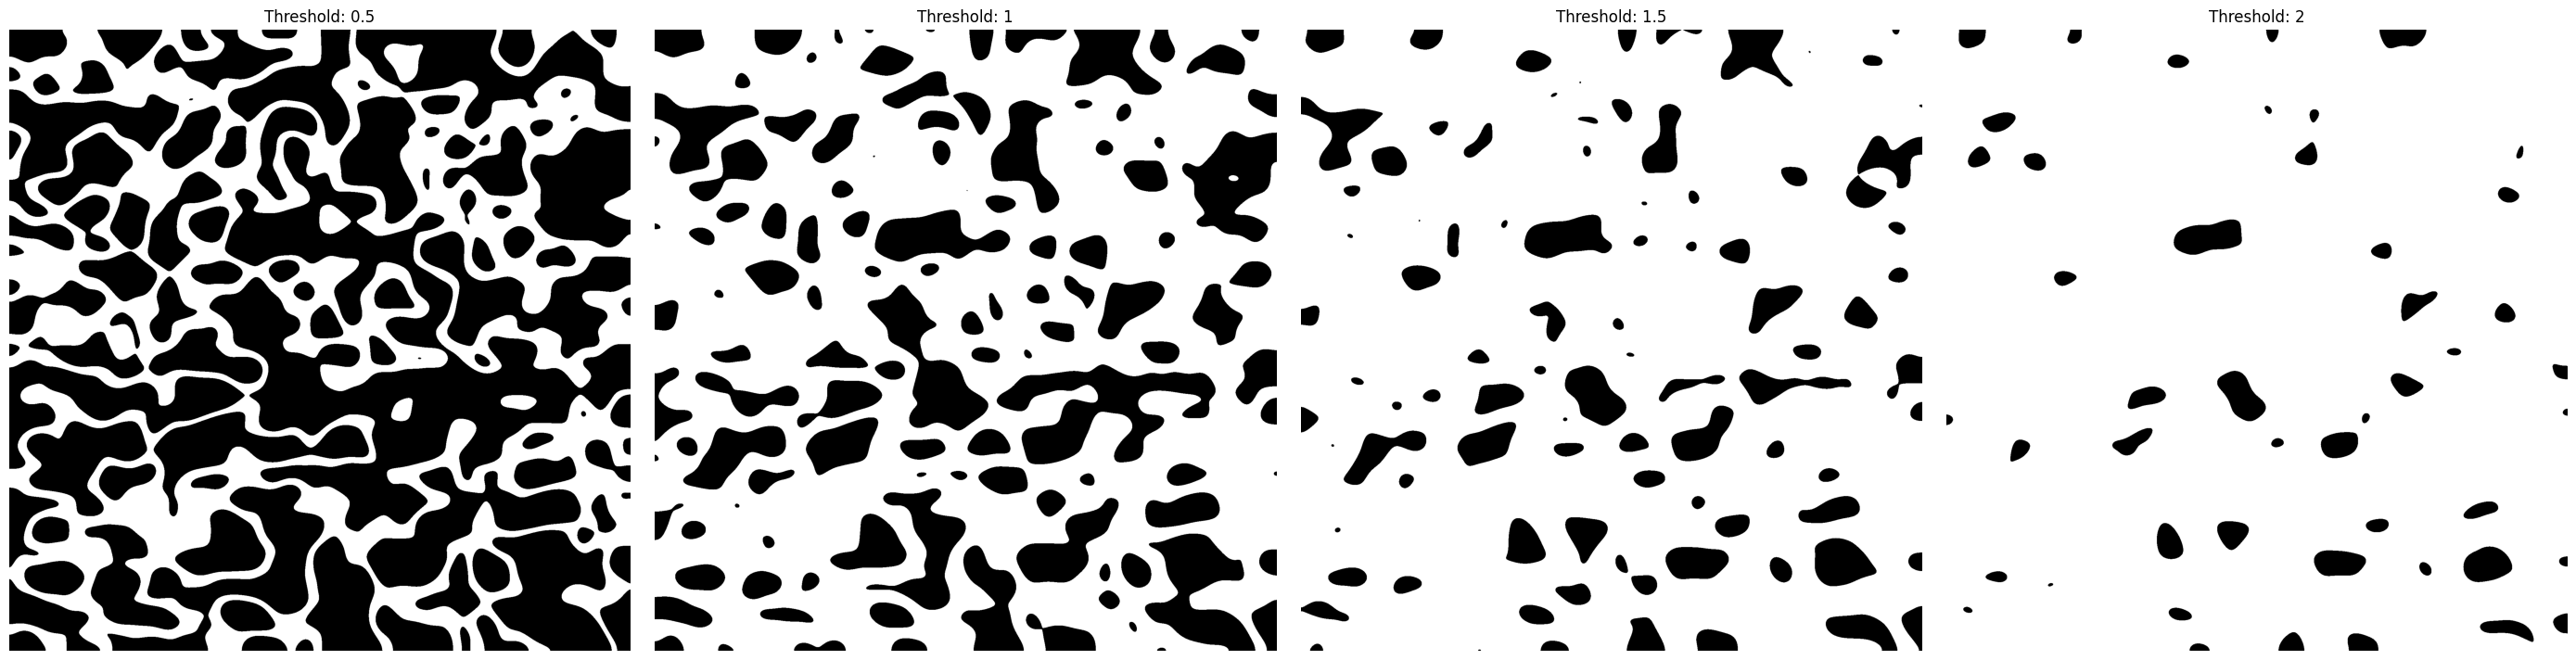
\includegraphics[width=\textwidth]{figures/threshold_comparison.png}
    \caption{Visualization of excursion sets $\Sigma(\nu) = \{ \kappa > \nu \sigma_0 \}$ of a two-dimensional random field $\kappa(\hat{\mathbf{n}})$, where $\kappa$ represents the convergence field with zero mean and variance $\sigma_0^2$. 
    Black regions correspond to regions where the field exceeds the threshold value $\nu \sigma_0$. The panels correspond to increasing threshold values ($\nu = 0.5, 1, 1.5, 2$), illustrating how the size and connectivity of the excursion sets change as the threshold increases.}
    \label{fig:excursion_sets}
\end{figure}
The three Minkowski functionals $V_0(\nu)$, $V_1(\nu)$, and $V_2(\nu)$ measure, respectively, the area, the length of the boundary, and the genus characteristic of these excursion sets:
\begin{align}
    V_0(\nu) &= \frac{1}{A} \int_{\Sigma(\nu)} \, da, \label{eq:minkowski_V0} \\
    V_1(\nu) &= \frac{1}{4A} \int_{\partial \Sigma(\nu)} \, dl, \label{eq:minkowski_V1} \\
    V_2(\nu) &= \frac{1}{2\pi A} \int_{\partial \Sigma(\nu)} \mathcal{K} \, dl, \label{eq:minkowski_V2}
\end{align}
where $A$ is the total area of the field, $da$ and $dl$ are the area and length elements, and $\mathcal{K}$ is the geodesic curvature along the boundary $\partial \Sigma(\nu)$. 

\begin{comment}
\subsection{Computation of Minkowski Functionals}
In practical applications, Minkowski functionals are computed numerically from discrete convergence maps.

For a given threshold $\nu$, the excursion set $\Sigma(\nu)$ is identified by:
\begin{equation}
    \Sigma(\nu) = \{ \hat{\mathbf{n}} \in S^2 \mid \tilde{\kappa}(\hat{\mathbf{n}}) > \nu \}, \label{eq:excursion_set_normalized}
\end{equation}
where $\tilde{\kappa} = (\kappa - \langle \kappa \rangle) / \sigma_0$ is the normalized convergence field.

Given a pixelized convergence map, the continuous integrals in Equations~\eqref{eq:minkowski_V0}--\eqref{eq:minkowski_V2} are approximated by discrete sums \citep{2012PhRvD..85j3513K}:
\begin{align}
    V_0(\nu) &\approx \frac{1}{N_{\mathrm{pix}}} \sum_{i=1}^{N_{\mathrm{pix}}} \Theta(\tilde{\kappa}_i - \nu), \label{eq:V0_discrete} \\
    V_1(\nu) &\approx \frac{1}{N_{\mathrm{pix}}} \sum_{i=1}^{N_{\mathrm{pix}}}  \delta_D(\tilde{\kappa}_i - \nu) \, \sqrt{\kappa_{, x}^2 + \kappa_{, y}^2}, \label{eq:V1_discrete} \\
    V_2(\nu) &\approx \frac{1}{N_{\mathrm{pix}}} \sum_{i=1}^{N_{\mathrm{pix}}}  \delta_D(\tilde{\kappa}_i - \nu) \, \frac{2\kappa_{, x}\kappa_{, y}\kappa_{, xy} - \kappa_{, x}^2 \kappa_{, yy} - \kappa_{, y}^2}{\kappa_{, xx}{\kappa_{, x}^2 + \kappa_{, y}^2}} \label{eq:V2_discrete}
\end{align}
where $\mathcal{N}(i)$ denotes the set of neighboring pixels to pixel $i$, and $\delta_D$ is the Dirac delta function. The first and second order derivatives $\kappa_{, x}$ etc., are approximated by finite differences.

\subsection{Minkowski Functionals in Gaussian Random Fields}
In the analysis of \emph{Gaussian random fields} (GRFs), Minkowski functionals provide a robust analytical framework for quantifying the morphological characteristics of the field's excursion sets. For a two-dimensional GRF \(\kappa(\hat{\mathbf{n}})\) with zero mean and variance \(\sigma_0^2\), the Minkowski functionals can be explicitly calculated and are given by \citep{2010PhRvD..81h3505M}:
\begin{align}
    V_0(\nu) &= \frac{1}{2}\left[1 - \mathrm{erf}\left( \frac{\nu}{\sqrt{2}\sigma_0} \right) \right], \label{eq:V0_GRF} \\
    V_1(\nu) &= \frac{1}{8\sqrt{2}} \frac{\sigma_1}{\sigma_0} \exp\left( -\frac{\nu^2}{2\sigma_0^2} \right), \label{eq:V1_GRF} \\
    V_2(\nu) &= \frac{\nu}{4\sqrt{2}} \frac{\sigma_1^2}{\sigma_0^3} \exp\left( -\frac{\nu^2}{2\sigma_0^2} \right), \label{eq:V2_GRF}
\end{align}
where \(\nu\) denotes the threshold level defining the excursion set, \(\mathrm{erf}\) is the error function, and \(\sigma_1^2 = \langle |\nabla \kappa|^2 \rangle = \langle \kappa_{, x}^2 + \kappa_{, y}^2 \rangle\) represents the variance of the gradient of the field. Here, \(V_0(\nu)\) corresponds to the area fraction of the excursion set, \(V_1(\nu)\) to the total boundary length per unit area, and \(V_2(\nu)\) to the Euler characteristic per unit area.

\subsection{Applications in Cosmology}
Minkowski functionals furnish an algebraic framework for quantifying the geometrical and topological properties of scalar fields \citep{1994A&A...288..697M}. In cosmology, they are instrumental in characterizing the intricate patterns formed by the large-scale structure of the Universe \citep{1996dmu..conf..281S, 1997ApJ...482L...1S}. These patterns, which trace the underlying matter distribution, are sensitive to higher-order statistical moments of the matter density field and thus provide insights beyond those accessible through two-point correlation functions \citep{2001ApJ...551L...5S}.

Recently, Minkowski functionals have been extensively employed in various cosmological investigations. They have been utilized to probe non-linear features in the CMB anisotropies \citep{2012JCAP...01..048L, 2016MNRAS.461.1363N, 2024JCAP...01..039C, 2024JCAP...05..076H}, to analyze anisotropies in the distribution of galaxies \citep{2003PASJ...55..911H, 2022ApJ...928..108A}, to constrain neutrino masses through their impact on the matter power spectrum \citep{2024MNRAS.528.4513M, 2023JCAP...09..037L}, and to test theories of modified gravity that predict deviations from General Relativity on cosmological scales \citep{2017MNRAS.466.2402S, 2024PhRvD.109h3537J}. Moreover, Minkowski functionals have emerged as a powerful and efficient probe for detecting primordial non-Gaussianity, as demonstrated in several studies \citep{2006ApJ...653...11H, 2008MNRAS.385.1613H, 2008MNRAS.389.1439H, 2012MNRAS.425.2187H, 2012ApJ...760...45S}.

In the realm of weak lensing, Minkowski functionals have been proposed as a method to break the degeneracy between the matter density parameter \(\Omega_m\) and the amplitude of matter fluctuations \(\sigma_8\) inherent in traditional two-point statistics \citep{2001ApJ...552L..89M}. Subsequent studies have leveraged Minkowski functionals applied to weak lensing convergence maps to extract cosmological information beyond that accessible through the power spectrum alone, thereby enhancing constraints on cosmological parameters \citep{2012PhRvD..85j3513K, 2013ApJ...774..111S, 2015PhRvD..91j3511P, 2022OJAp....5E..13G}.
\end{comment}